\chapter{\IfLanguageName{dutch}{Stand van zaken}{State of the art}}%
\label{ch:stand-van-zaken}

% Tip: Begin elk hoofdstuk met een paragraaf inleiding die beschrijft hoe
% dit hoofdstuk past binnen het geheel van de bachelorproef. Geef in het
% bijzonder aan wat de link is met het vorige en volgende hoofdstuk.

% Pas na deze inleidende paragraaf komt de eerste sectiehoofding.

% Dit hoofdstuk bevat je literatuurstudie. De inhoud gaat verder op de inleiding, maar zal het onderwerp van de bachelorproef *diepgaand* uitspitten. De bedoeling is dat de lezer na lezing van dit hoofdstuk helemaal op de hoogte is van de huidige stand van zaken (state-of-the-art) in het onderzoeksdomein. Iemand die niet vertrouwd is met het onderwerp, weet nu voldoende om de rest van het verhaal te kunnen volgen, zonder dat die er nog andere informatie moet over opzoeken \autocite{Pollefliet2011}.

% Je verwijst bij elke bewering die je doet, vakterm die je introduceert, enz.\ naar je bronnen. In \LaTeX{} kan dat met het commando \texttt{$\backslash${textcite\{\}}} of \texttt{$\backslash${autocite\{\}}}. Als argument van het commando geef je de ``sleutel'' van een ``record'' in een bibliografische databank in het Bib\LaTeX{}-formaat (een tekstbestand). Als je expliciet naar de auteur verwijst in de zin (narratieve referentie), gebruik je \texttt{$\backslash${}textcite\{\}}. Soms is de auteursnaam niet expliciet een onderdeel van de zin, dan gebruik je \texttt{$\backslash${}autocite\{\}} (referentie tussen haakjes). Dit gebruik je bv.~bij een citaat, of om in het bijschrift van een overgenomen afbeelding, broncode, tabel, enz. te verwijzen naar de bron. In de volgende paragraaf een voorbeeld van elk.

% \textcite{Knuth1998} schreef een van de standaardwerken over sorteer- en zoekalgoritmen. Experten zijn het erover eens dat cloud computing een interessante opportuniteit vormen, zowel voor gebruikers als voor dienstverleners op vlak van informatietechnologie~\autocite{Creeger2009}.

% Let er ook op: het \texttt{cite}-commando voor de punt, dus binnen de zin. Je verwijst meteen naar een bron in de eerste zin die erop gebaseerd is, dus niet pas op het einde van een paragraaf.

In de context van hedendaags onderzoek naar de veehouderij is de integratie van sensortechnologie en kunstmatige intelligentie (AI) van cruciaal belang. 
Deze technologieën spelen een sleutelrol in het verbeteren van zowel de efficiëntie en nauwkeurigheid van veebewaking als het bevorderen van hogere normen van dierenwelzijn en ethische landbouwpraktijken \autocite{PastureIo}.
\section{Achtergrond en belang van monitoringssystemen in de veehouderij}
De transitie van traditionele naar moderne methoden in het monitoren van vee markeert een significante vooruitgang in de agrarische sector. Terwijl monitoringssystemen vroeger voornamelijk een arbeidsintensief proces was met visuele observatie en manuele registratie, heeft de introductie van technologische innovaties deze processen efficiënter, nauwkeuriger en kosten-effectiever gemaakt\autocite{ToAgriculture}. Deze technologische vooruitgang is met name merkbaar in de implementatie van Internet of Things (IoT) technologieën, die een geïntegreerde aanpak bieden voor het beheer van vee\autocite{IntuzIoT}.
\newline
Één  van de voornaamste voordelen van moderne veebeheer is de aanzienlijke verbetering van dierenwelzijn. Dit wordt bereikt door het vroegtijdig detecteren van ziektes en verwondingen, waardoor preventieve of corrigerende maatregelen kunnen worden genomen voordat deze problemen ernstig worden. Dergelijke monitoring stelt boeren in staat om de fok- en voedingscycli van dieren nauwlettend te volgen, wat resulteert in betere reproductieve prestaties en hogere productiviteit\autocite{ToAgriculture}.
\newline
De toegenomen rendabiliteit is een ander belangrijk voordeel van geavanceerde monitoringssystemen. Door continu de gezondheid, het gedrag en de locatie van dieren te monitoren, 
kunnen boeren beter geïnformeerde beslissingen nemen over fokken, voeren en grazen. Dit resulteert niet alleen in hoogwaardigere producten, maar leidt ook tot hogere opbrengsten en verhoogde winsten voor de boerderij\autocite{ToAgriculture}. 
Bovendien biedt IoT-technologie gedetailleerde real-time gegevens over de dieren, wat essentieel is voor een effectieve veehouderij\autocite{IntuzIoT}.
\newline
Het gebruik van technologie in veebeheer heeft ook geleid tot aanzienlijke kostenbesparingen. 
Door middel van efficiënte resource management, zoals voeder- en waterbeheer, kunnen boeren geld besparen en tegelijkertijd de duurzaamheid van hun boerderijen verbeteren. 
Vroege detectie van ziektes helpt ook bij het verminderen van dure dierenartskosten en het verlies van vee\autocite{ToAgriculture}\autocite{IntuzIoT}.
\newline
Ondanks deze voordelen zijn er ook uitdagingen en beperkingen verbonden aan het implementeren van technologie-gebaseerde monitoringssystemen. De kosten en complexiteit van dergelijke systemen, evenals privacy- en beveiligingszorgen, vormen significante hindernissen. 
Daarnaast is er vaak behoefte aan gespecialiseerde training en deskundigheid om deze systemen effectief te gebruiken en te integreren met bestaande boerderij management systemen\autocite{ToAgriculture}\autocite{IntuzIoT}.
\newline

\section{AI technieken in de landbouw}
Kunstmatige intelligentie (AI) heeft een revolutie teweeggebracht in de landbouw, met bijzondere nadruk op het gebruik van detectietechnieken voor het monitoren van vee en gewassen. 
Deze technologieën stellen landbouwers in staat om nauwkeurige data-analyses uit te voeren, wat leidt tot betere besluitvorming in gewasbeheer en dierverzorging. AI-toepassingen variëren van ziekteherkenning bij planten tot gedragsanalyse bij dieren, en spelen een sleutelrol in precisielandbouw \autocite{jafar2024revolutionizing}.
Hieronder worden verschillende AI-technieken besproken die in de landbouw worden toegepast.

\subsection{Machine learning}
Machine Learning-algoritmes worden breed toegepast voor het analyseren van enorme datasets. Ze zijn bijzonder vaardig in het identificeren van patronen en correlaties in data die niet direct waarneembaar zijn voor mensen. Dit heeft geleid tot verbeterde voorspellingen over gewasopbrengsten, optimalisatie van bemestingsschema's en vroegtijdige detectie van ziekten en plagen in gewassen \autocite{morota2018machine}.

\subsection{De rol van beeldherkenning}
De rol van beeldherkenning en computer vision in de landbouw is eveneens van onschatbare waarde. Met de inzet van camera's en drones worden beelden van velden en gewassen verzameld en geanalyseerd. Deze techniek is cruciaal voor het detecteren van de gezondheid van gewassen, het identificeren van onkruid, ziekten en plagen, en draagt bij aan een preciezere identificatie van problemen in gewassen. Dit leidt tot gerichtere behandelingen en vermindert de verspilling van pesticiden en nutriënten aanzienlijk \autocite{morota2018big}.

\subsection{Predictieve analyse}
Predictieve analyse, vaak gevoed door machine learning-modellen, speelt een belangrijke rol in het voorspellen van toekomstige omstandigheden in de landbouw. Deze technieken maken gebruik van zowel historische data als real-time informatie om voorspellingen te doen over weersomstandigheden, ziekte-uitbraken of markttrends. De inzet van predictieve analyse in de landbouw leidt tot een betere voorbereiding op toekomstige omstandigheden, efficiëntere planning en verbeterd risicobeheer \autocite{akhter2022precision}.
\subsection{Conclusie}
Deze AI-technieken vormen de basis van wat nu bekend staat als precisielandbouw. Ze stellen boeren in staat om hun bedrijfsvoering te optimaliseren door meer nauwkeurige inzichten en voorspellingen te bieden. De voortdurende ontwikkeling en verfijning van deze technieken zullen ongetwijfeld leiden tot verdere verbeteringen in de landbouwsector. De toekomst van landbouw ziet er dankzij AI helder uit, met voordelen zoals hogere opbrengsten, duurzamere praktijken en een beter begrip van het complexe ecosysteem waarin de landbouw opereert \autocite{bhat2021big}.

\section{Beeldherkenning en -verwerking in de landbouw}
De integratie van AI in beeldherkenning en -verwerking is een doorslaggevend element geworden in vele technologische toepassingen. Elk algoritme achter deze technologieën heeft zijn eigen uniek mechanisme en toepassingsgebied.

\subsection{Convolutional neural networks (CNNs)}
CNN's zijn gespecialiseerd in het analyseren van visuele beelden door het gebruik van convolutionele lagen (zie figuur \ref{fig:standvanzaken_cnn}) die patronen en kenmerken in de afbeeldingen filteren en identificeren. Deze lagen kunnen variëren in complexiteit en zijn getraind om verschillende aspecten van de afbeelding te herkennen - van basale lijnen en randen tot complexere patronen zoals texturen en vormen. CNN's zijn bijzonder effectief in het classificeren en identificeren van objecten binnen afbeeldingen, dankzij hun vermogen om uitgebreide hiërarchieën van kenmerken te leren en te herkennen \autocite{sharma2018analysis}.
\newline
\begin{figure}[H]
  \centering
  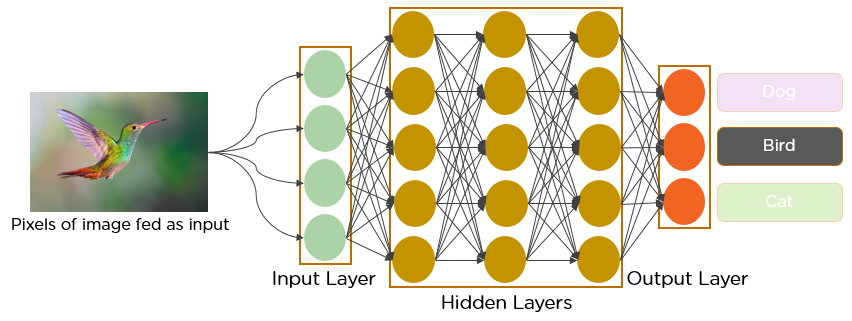
\includegraphics[width=\linewidth]{standvanzaken_cnn.png}
  \caption{Voorbeeld werking van CNN model. \cite{birdcnnimage2021}}
  \label{fig:standvanzaken_cnn}  
\end{figure}
\newline
\subsection{Region-based convolutional neural networks (R-CNNs)}
R-CNNs bouwen voort op de basis van CNN's en voegen een extra laag van complexiteit en precisie toe. Ze gebruiken 'region proposal'-algoritmes om interessante delen van de afbeelding te identificeren (zie figuur \ref{fig:standvanzaken_rcnn}) voordat ze deze door een CNN voeren voor classificatie. Dit proces resulteert in een nauwkeurigere en gerichte objectdetectie, omdat het algoritme zich richt op specifieke delen van de afbeelding die waarschijnlijker objecten bevatten. Dit maakt R-CNNs bijzonder geschikt voor toepassingen waarbij precisie in objectdetectie essentieel is \autocite{zhang2014part}.
Deze techniek is bijzonder nuttig in toepassingen zoals stadsplanning, waarbij R-CNNs worden ingezet om voertuigen en voetgangers op luchtfoto's van verkeersknooppunten te identificeren.
\newline
\begin{figure}[H]
  \centering
  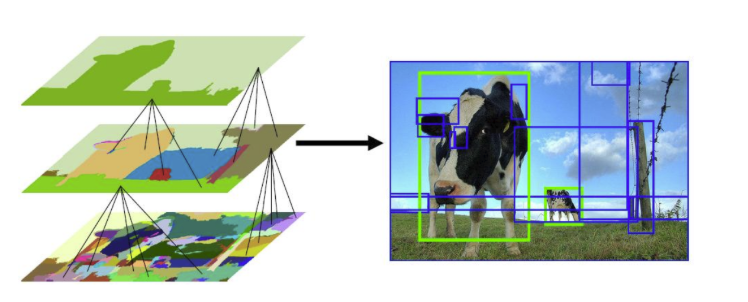
\includegraphics[width=\linewidth]{standvanzaken_rcnn.png}
  \caption{Voorbeeld van objectdetectie met R-CNN. \cite{towardsdatascience_rcnn}}
  \label{fig:standvanzaken_rcnn}  
\end{figure}
\newline
\subsection{YOLO (You Only Look Once)}
YOLO heeft een baanbrekende verandering teweeggebracht in de wereld van objectdetectie binnen computer vision. Dit algoritme wijkt af van de traditionele methodes, die vaak gebaseerd zijn op Convolutional Neural Networks (CNNs) en meerdere stappen omvatten, zoals het voorstellen van kandidaatregio's gevolgd door hun classificatie. YOLO daarentegen benadert objectdetectie als een enkelvoudig regressieprobleem dat direct van beeldpixels naar coördinaten van begrenzingsvakken en klassewaarschijnlijkheden gaat.
\newline
Het hart van YOLO is een CNN dat het hele beeld in één keer analyseert. Het beeld wordt verkleind naar een vast formaat en opgedeeld in een SxS raster (zie figuur \ref{fig:standvanzaken_yolo}). Elke cel in dit raster voorspelt meerdere begrenzingsvakken. Elk van deze vakken bevat zowel afmetingen als een betrouwbaarheidsscore, die de waarschijnlijkheid aangeeft dat het vak een object bevat. Tegelijkertijd voorspelt het model de klassewaarschijnlijkheid voor elke cel, die dan vermenigvuldigd wordt met de betrouwbaarheidsscore om de uiteindelijke voorspelling te doen.
\newline
De voornaamste kracht van YOLO ligt in zijn verwerkingsnelheid, waardoor het uitermate geschikt is voor real-time toepassingen zoals bewakingssystemen en autonome voertuigen. Deze snelheid komt soms ten koste van de nauwkeurigheid, vooral vergeleken met complexere modellen die in twee stappen werken. Desalniettemin heeft YOLO een aanzienlijke impact op het gebied van computer vision door aan te tonen dat effectieve en snelle objectdetectie mogelijk is door CNNs op een innovatieve manier te gebruiken binnen een gestroomlijnd framework \autocite{diwan2023object}.
\newline
\begin{figure}[H]
  \centering
  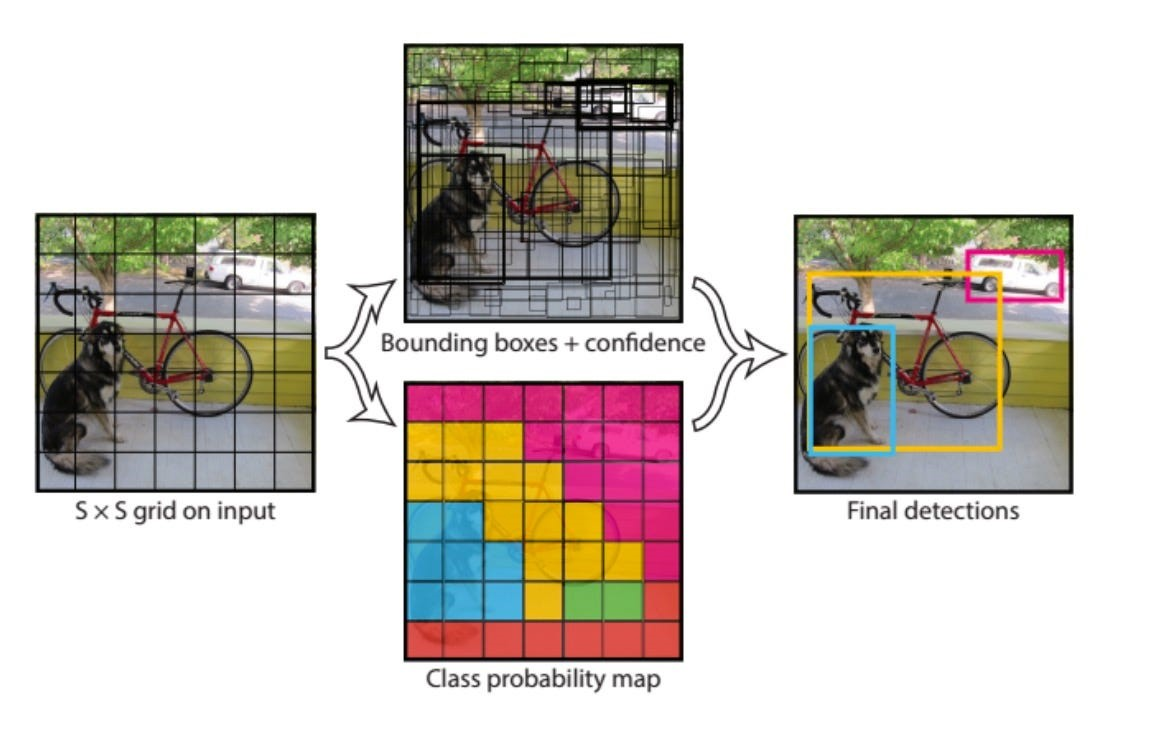
\includegraphics[width=\linewidth]{standvanzaken_yolo.jpg}
  \caption{Voorbeeld van objectdetectie met YOLO. \cite{springer_image}}
  \label{fig:standvanzaken_yolo}  
\end{figure}
\newline
\subsection{Pose estimation}
Pose estimation, een cruciaal onderdeel van computer vision, heeft een transformatie ondergaan dankzij moderne technologieën. Traditionele methoden, afhankelijk van markers en meervoudige camera's, zijn vervangen door geavanceerde diepe leermodellen. Deze modellen, vaak gebaseerd op Convolutional Neural Networks (CNN's) en nieuwere netwerkarchitecturen zoals Transformer-modellen, detecteren en lokaliseren sleutelpunten op het menselijk lichaam om houdingen te analyseren (zie figuur \ref{fig:standvanzaken_poseestimation}). Dit vermogen heeft brede toepassingen, variërend van interactieve games tot sportanalyse en gezondheidszorg.
De nieuwste systemen kunnen in real-time menselijke bewegingen accuraat herkennen, een vooruitgang die de interactie tussen mens en computer aanzienlijk verbetert. Hoewel uitdagingen zoals het herkennen van gedeeltelijk verborgen lichaamsdelen blijven bestaan, evolueert het veld voortdurend, met onderzoek gericht op het verbeteren van nauwkeurigheid en robuustheid. Pose estimation blijft een snelgroeiend en invloedrijk domein in computer vision \autocite{zheng2020deep}.
\newline
\begin{figure}[H]
  \centering
  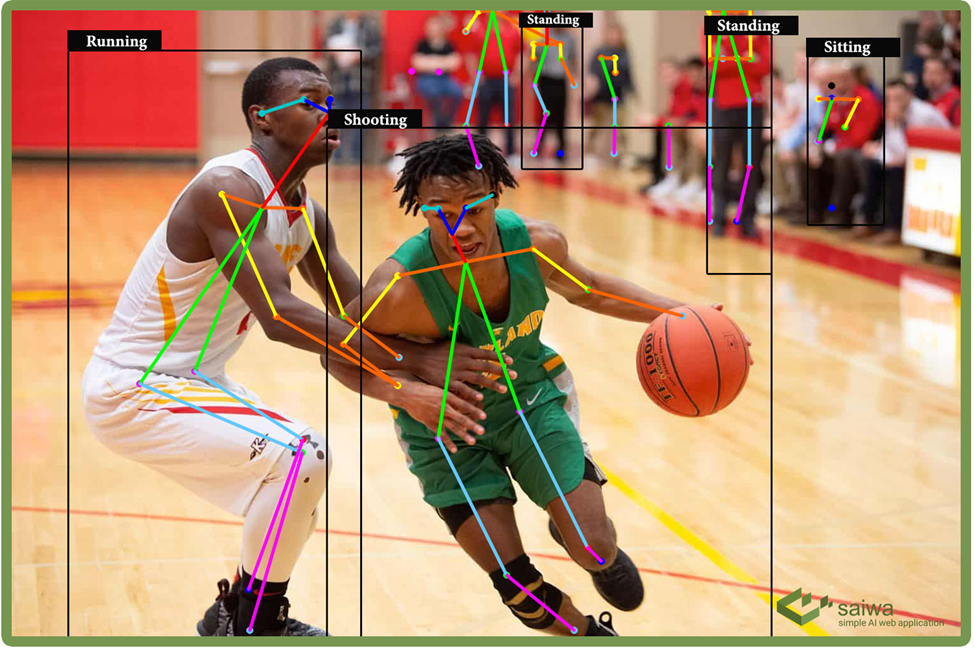
\includegraphics[width=\linewidth]{standvanzaken_poseestimation.png}
  \caption{Voorbeeld van pose estimation. \cite{medium_human_pose}.}
  \label{fig:standvanzaken_poseestimation}  
\end{figure}
\newline
\subsection{SSD (Single shot multiBox detector)}
SSD is een efficiënt objectdetectie-algoritme dat gebruikmaakt van één enkel diep neuraal netwerk, gebaseerd op Convolutional Neural Networks (CNNs). 
Het is ontworpen om objecten van verschillende groottes snel en nauwkeurig te identificeren door het genereren van feature maps op verschillende schaalniveaus. 
SSD voegt extra convolutielagen toe aan een basis-CNN om detecties uit te voeren op meerdere schalen, waardoor het zowel kleine als grote objecten effectief kan detecteren. 
Voor elke locatie in deze feature maps produceert het meerdere bounding boxes met bijbehorende classificatiescores. 
Door zijn snelle en nauwkeurige detectievermogen is SSD bijzonder geschikt voor real-time toepassingen (zie figuur \ref{fig:standvanzaken_SSD}) \autocite{kumar2020object}.
\newline
\begin{figure}[H]
  \centering
  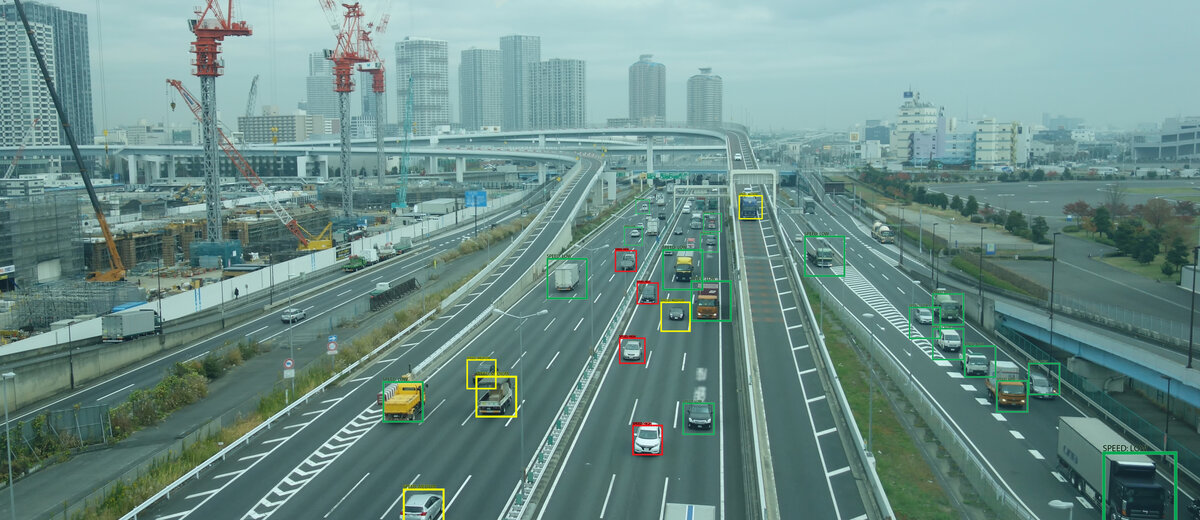
\includegraphics[width=\linewidth]{standvanzaken_object-detection-mobile-ssd.jpg}
  \caption{Voorbeeld van objectdetectie met SSD. \cite{automatic_addison_mobilenet}}
  \label{fig:standvanzaken_SSD}  
\end{figure}
\newline
\subsection{Feature detection (SIFT, SURF, ORB, etc.)}
Feature detection-algoritmes zoals SIFT (Scale-Invariant Feature Transform), SURF (Speeded-Up Robust Features), en ORB (Oriented FAST and Rotated BRIEF) zijn cruciaal voor het identificeren van specifieke punten of kenmerken binnen een afbeelding die invariant zijn voor schaal, rotatie en soms belichting (zie figuur \ref{fig:standvanzaken_featurematching}). Deze technieken zijn essentieel in beeldverwerking voor het vinden van overeenkomsten tussen verschillende afbeeldingen, bijvoorbeeld voor beeldregistratie en objecttracking \autocite{tareen2018comparative}.

\subsection{Feature matching (FLANN)}
FLANN staat voor Fast Library for Approximate Nearest Neighbors en is een algoritme dat gebruikt wordt voor het snel vinden van dichtstbijzijnde matches van features tussen verschillende sets van gegevens. Dit is bijzonder nuttig in combinatie met feature detection-algoritmes, omdat het helpt bij het efficiënt matchen van kenmerken tussen verschillende beelden, wat essentieel is voor taken zoals 3D-reconstructie, tracking en beeldstitching (zie figuur \ref{fig:standvanzaken_featurematching}) \autocite{Cong2016fast}.
\newline
\begin{figure}[H]
  \centering
  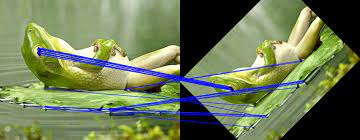
\includegraphics[width=\linewidth]{standvanzaken_featurematching.png}
  \caption{Voorbeeld van feature detection en matching tussen twee gedraaide afbeeldingen. \cite{haskell_opencv}}
  \label{fig:standvanzaken_featurematching}  
\end{figure}
\newline

\section{Huidige technieken voor diermonitoring}
In de hedendaagse landbouw spelen geavanceerde localisatietechnieken een cruciale rol in het effectief beheer van vee. Deze technologieën, variërend van satellietnavigatiesystemen tot op RFID-gebaseerde trackers, dragen bij aan de nauwkeurigheid en efficiëntie van monitoringssystemen in de veehouderij. In deze sectie worden enkele van deze technologieën en hun toepassingen besproken \autocite{halachmi2019smart}.

\subsection{Global positioning system (GPS)}
Global Positioning System is een technologie die boeren helpt bij het volgen van hun vee met behulp van satellieten. 
Denk aan het GPS-systeem in auto's, maar dan voor koeien. Met GPS kunnen boeren precies zien waar hun dieren zich bevinden op grote, open weidegronden, waar het moeilijk is om ze in de gaten te houden. 
Dit is niet alleen handig om het vee te localiseren, maar het helpt ook bij het beheren van het land. Door te zien waar de dieren grazen, kunnen boeren overbegrazing voorkomen, wat zowel goed is voor het milieu als voor de gezondheid van het vee​​ \autocite{handcock2009monitoring}.
\begin{figure}[H]
  \centering
  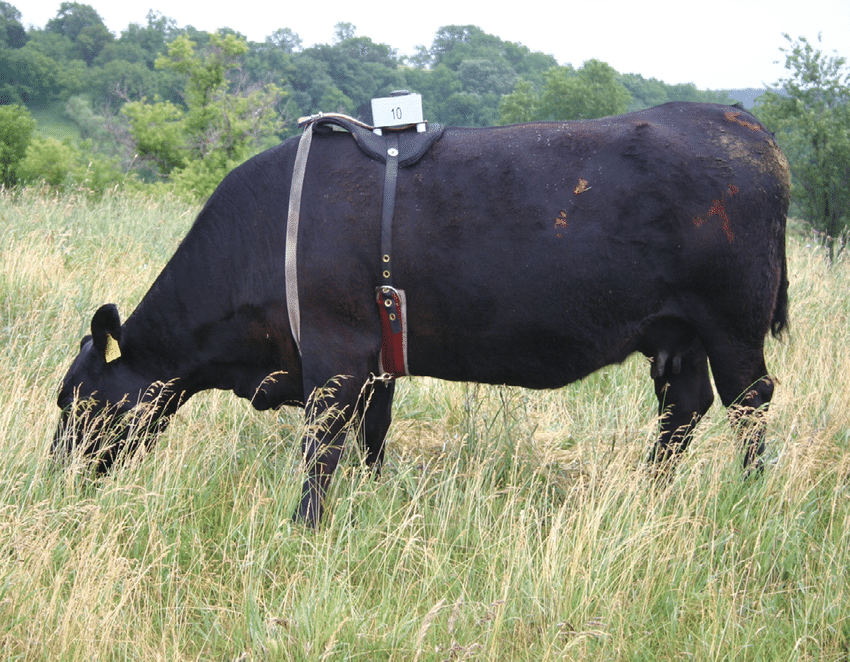
\includegraphics[width=\linewidth]{standvanzaken_gps.png}
  \caption{Voorbeeld van GPS-tracking van vee. \cite{researchgate_cow_gps}}
  \label{fig:standvanzaken_gps}  
\end{figure}
\subsection{Real-time kinematic (RTK) GPS-systemen}
Een geavanceerde variant van GPS-technologie is het Real-Time Kinematic (RTK) GPS-systeem. RTK-GPS biedt een aanzienlijk hogere nauwkeurigheid dan traditionele GPS-systemen door gebruik te maken van vaste referentiestations. Deze stations zenden correctiesignalen uit die de locatiegegevens van het GPS-systeem verfijnen. Voor veehouderij betekent dit dat boeren de positie van hun vee of machines kunnen volgen met een precisie tot op enkele centimeters (zie figuur \ref{fig:standvanzaken_rtk}). Dit niveau van nauwkeurigheid is cruciaal, bijvoorbeeld voor het monitoren van gedragspatronen of het nauwkeurig beheren van weidegronden. De implementatie van RTK-GPS in de veehouderij draagt bij aan een nog efficiëntere bedrijfsvoering en kan helpen bij het verbeteren van dierenwelzijn door gedetailleerder inzicht in het gedrag van het vee \autocite{keshavarzi2021validation}.
\begin{figure}[H]
  \centering
  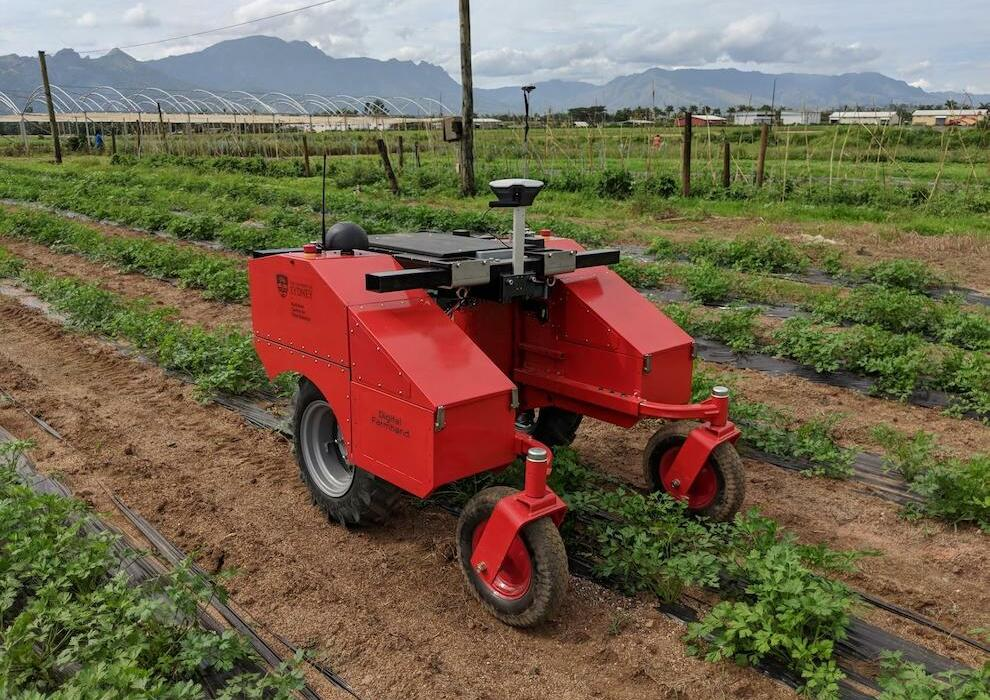
\includegraphics[width=\linewidth]{standvanzaken_rtk.jpg}
  \caption{Voorbeeld van een RTK (Real Time Kinematic) GPS-ontvanger in gebruik binnen een landbouwomgeving, getoond met een Emlid Reach receiver. \cite{emlid2019agrobot}}
  \label{fig:standvanzaken_rtk}  
\end{figure}
\subsection{Radiofrequentie-identificatie (RFID)}
Radiofrequentie-identificatie heeft zich gevestigd als een belangrijke technologie in de moderne veehouderij. 
RFID-technologie wordt gebruikt om individuele dieren te identificeren en te volgen, waarbij dieren worden uitgerust met RFID-oorlabels die door zowel draagbare als vaste lezers kunnen worden uitgelezen. Deze technologie stelt boeren in staat om vee-inventarisatie efficiënt uit te voeren en essentiële gezondheidsgegevens van elk dier te registreren. \autocite{voulodimos2009complete}
Daarnaast moedigen overheden wereldwijd het gebruik van deze technologie aan voor beter beheer van dierziekten. 
In de Verenigde Staten bijvoorbeeld, overweegt het ministerie van Landbouw (USDA) het gebruik van RFID-tags verplicht te stellen voor al het vee dat bij internationale reizen en tentoonstellingen betrokken is​​. \autocite{rfidjournal2024rfid}

\subsection{Draadloze sensor netwerken (WSN)}
Draadloze Sensor Netwerken zijn cruciaal in de hedendaagse precisielandbouw, vooral in de context van veehouderij. Deze technologie bestaat uit een netwerk van kleine, draadloze sensoren die strategisch over een landbouwgebied worden verspreid om een veelheid aan gegevens te verzamelen. Deze sensoren kunnen diverse omgevingsparameters meten, zoals temperatuur, luchtvochtigheid en bodemgesteldheid, evenals dierlijke bewegingen en gedragingen. Integratie van WSN met andere technologieën zoals GPS en RFID biedt een holistisch beeld van zowel de vee- als omgevingscondities \autocite{oja2015wireless}.

\subsection{Conclusie}
In de praktijk transformeren deze technologieën de manier waarop boeren hun vee beheren. Bijvoorbeeld, door gebruik te maken van GPS en RFID, kunnen boeren de locatie van hun vee volgen, terwijl WSN cruciale gegevens over hun gezondheid en welzijn levert. Deze geïntegreerde aanpak leidt tot betere besluitvorming en optimaliseert de algehele boerderijefficiëntie. Case studies tonen aan dat dergelijke technologieën helpen bij het verminderen van arbeidskosten, het verhogen van de productiviteit en het verbeteren van dierenwelzijn \autocite{mohamed2021smart}.


\section{Relevant onderzoek en case studies}
\newline
AI en sensortechnologieën brengen een significante verandering in de zuivelsector, gericht op uitdagingen zoals ziektecontrole en dierenwelzijn. Deze technologieën maken real-time monitoring en datagedreven besluitvorming mogelijk, wat leidt tot beter dierenwelzijn en efficiëntere supply chain operaties. Belangrijke toepassingen zijn de identificatie van minder assertieve koeien tijdens het voeden en de automatisering van gewichtsregistratie. Uitdagingen omvatten onderhoud van sensoren, databeveiliging en economische overwegingen. Toekomstige ontwikkelingen in AI en sensortechnologieën dragen bij aan duurzamere en meer geoptimaliseerde veehouderijpraktijken, hoewel ze nieuwe uitdagingen zoals dataprivacy met zich meebrengen. 
AI en sensortechnologieën zijn cruciaal voor een toekomstige veehouderij die zich richt op efficiëntie, duurzaamheid en humaan beheer, met verbeteringen in ziekteherkenning en voedingsstrategieën \autocite{MDPIAIandSensors}.
% \newline
% Een ander belangrijk concept binnen deze context is Precision Livestock Farming (PLF), dat gebruikmaakt van informatietechnologie voor real-time monitoring en beheer van vee. 
% Door de implementatie van geavanceerde technologieën zoals microfluidica en geluidsanalyse, heeft PLF geleid tot aanzienlijke verbeteringen in de nauwkeurigheid van gezondheidsmonitoring \autocite{MDPIPLF}.
\newline
In de studie \textcite{Fuentes2023}, wordt de inzet van diepgaand leren voor het monitoren van individueel koeiengedrag binnen de context van precisieveehouderij (PLF) onderzocht. Deze aanpak is specifiek gericht op Hanwoo vee, een inheemse Koreaanse veesoort, en maakt gebruik van een netwerk van CCTV-camera's in een gesloten boerderij. Door het analyseren van RGB-videobeelden, identificeert en volgt het systeem verschillende acties van het vee, wat bijdraagt aan een grondige lange-termijn gedragsanalyse.

De studie toont aan dat, ondanks uitdagingen zoals veranderingen in grootte van de dieren, bewegingsvariatie, en occlusie, het systeem effectief individuele koeien kan herkennen en hun gedrag kan monitoren. Dit resulteert in waardevolle inzichten in de gezondheid, emoties, en het welzijn van de dieren, wat cruciaal is voor geavanceerde PLF-praktijken.

De bevindingen van de studie onderstrepen het potentieel van AI en deep learning voor het verbeteren van PLF door niet-intrusieve, continue monitoring van veegedrag in een gecontroleerde omgeving. Deze methodologie biedt significante voordelen voor de veehouderij, vooral in termen van verbeterd dierenwelzijn en efficiëntie. De resultaten van dit onderzoek bieden belangrijke inzichten en vormen een waardevolle toevoeging aan de bestaande literatuur over de toepassing van technologie in de moderne veehouderij.
% \newline
% Het gebruik van sensoren en draagbare technologieën voor vroege ziekteopsporing bij vee zijn essentieel voor het verbeteren van de efficiëntie en effectiviteit van landbouwbedrijven en bieden mogelijkheden voor tijdige interventies en verbeterd beheer \autocite{Animals13780}.
\newline
In het onderzoek van \textcite{ar5iv2021} ontwikkelden ze een nieuwe manier om met behulp van deep learning het gedrag van dieren te analyseren, specifiek gericht op vee dat een slimme halsband draagt (zie figuur \ref{fig:standvanzaken_koeiensensor}). Deze halsbanden, uitgerust met versnellingsmeters, verzamelen data over hoe de dieren zich bewegen. Het slimme aan de halsbanden is dat ze het gedrag van de dieren, zoals lopen, grazen of rusten, direct kunnen herkennen en classificeren.
Deze methode is bijzonder omdat het makkelijker en efficiënter is dan de traditionele manieren van gedragsobservatie, zoals het handmatig volgen van dieren of het gebruik van camera’s en microfoons. Bovendien werkt deze technologie in real-time en legt het geen grote druk op de batterij of het geheugen van de halsband. Dit is erg handig voor boeren, omdat ze zo beter inzicht krijgen in het welzijn en de gezondheid van hun vee, zonder veel extra moeite of technische complexiteit. De onderzoekers hebben hun systeem getest met koeien in de wei en ontdekten dat het heel nauwkeurig verschillende gedragingen kon identificeren, wat het een veelbelovende tool maakt voor moderne veeteelt.
\newline
\begin{figure}[H]
  \centering
  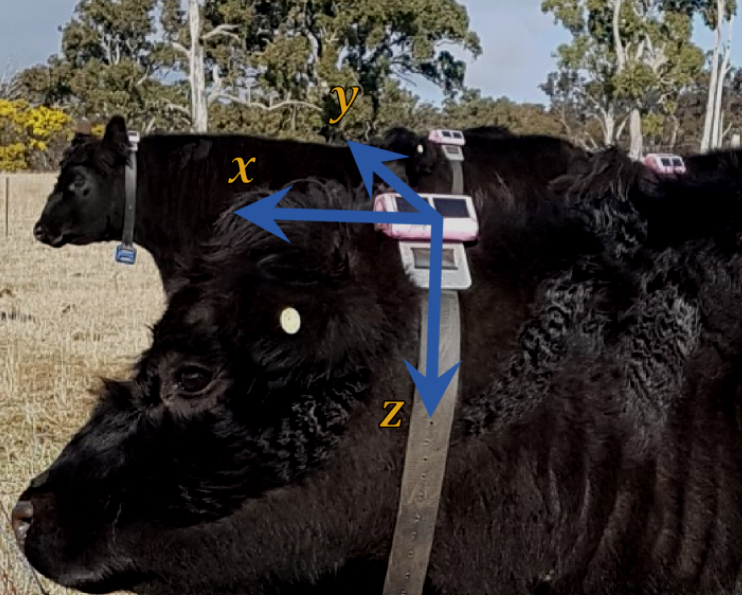
\includegraphics[width=\linewidth]{standvanzaken_koeiensensor.png}
  \caption{Voorbeeld van een slimme halsband voor koeien. \cite{ar5iv2021}}
  \label{fig:standvanzaken_koeiensensor}  
\end{figure}
\newline
Samengevat illustreren deze onderzoeken de impact van deep learning, biosensoren, en machine learning in de veehouderij. 
Deze technologieën verbeteren niet alleen het veebeheer en het welzijn van de dieren, maar dragen ook significant bij aan duurzamere landbouwpraktijken. 
De combinatie van data van zowel draagbare sensoren als omgevingsensoren, samen met de toepassing van diepe leeralgoritmen, zou kunnen leiden tot een nog uitgebreider begrip van de gezondheid en het welzijn van vee en de verdere ontwikkeling van duurzame veehouderijpraktijken.
\section{Voordelen van mijn methode in koeiengedrag identificatie en localisatie}
De methode die in mijn bachelorproef wordt toegepast, onderscheidt zich van bestaande onderzoeken op het gebied van veemonitoring en -gedragsanalyse. 
Door het integreren en vergelijken van geavanceerde technologieën van object detectie en classificatie, animal pose estimation en een unieke combinatie van GPS-gegevens met camera perspectief transformatie, biedt deze aanpak verbeteringen in nauwkeurigheid, efficiëntie en het begrip van koeiengedrag in de landbouw.
\subsection{Integratie van deep learning en animal pose estimation}
Traditioneel richten onderzoeken, zoals dat van \textcite{Fuentes2023} zich op het gebruik van CCTV-camera’s en diepgaand leren voor de monitoring van vee, maar ze missen de gelaagdheid die animal pose estimation biedt. 
Mijn methode, die object classificatie combineert met animal pose estimation, gaat een stap verder en maakt het mogelijk om subtiele gedragspatronen en fysieke houdingen van koeien te analyseren. 
Deze combinatie biedt niet alleen een algemene monitoring, maar stelt ons ook in staat om gedetailleerd gedrag zoals eten, rusten, of sociale interacties nauwkeurig te identificeren, wat cruciaal is voor het begrijpen van dierenwelzijn en gezondheid.
\subsection{Geavanceerde localisatietechnieken}
In tegenstelling tot de standaard GPS-tracking methoden zoals gebruikt in de onderzoeken \textcite{halachmi2019smart}, introduceert mijn methode een innovatieve dimensie in de localisatie van vee met het gebruik van camera perspectief transformatie in combinatie met GPS. 
Deze techniek levert niet alleen real-time locatiegegevens, maar biedt ook essentiële contextuele informatie over de omgeving van de dieren. Verder, in contrast met studies zoals die \textcite{Fuentes2023}, die zich richten op gedragsclassificatie in afgesloten omgevingen zoals stallen, breidt mijn onderzoek de toepasbaarheid uit naar open velden. Deze uitgebreide benadering maakt het mogelijk om koeien te observeren en te volgen in uitgestrekte weidegebieden, waardoor rijkere contextuele inzichten over hun interacties en gedragspatronen in een natuurlijke, minder restrictieve omgeving verkregen worden. 
Dit draagt significant bij aan een realistischer en completer begrip van koeiengedrag, wat fundamenteel is voor de effectiviteit en duurzaamheid van moderne veehouderijpraktijken.
\subsection{Conclusie}
Mijn methode biedt een omvattende en innovatieve benadering voor de studie van koeiengedrag en -localisatie. Door verschillende technologieën te testen, integreren en toe te passen in zowel beperkte als open omgevingen, overbrugt deze methode de kloof tussen traditionele monitoringstechnieken en moderne, geavanceerde technologieën. Dit biedt niet alleen een nauwkeurigere en efficiëntere manier om vee te monitoren, maar biedt ook nieuwe mogelijkheden voor onderzoek en toepassing in de precisielandbouw.